% !TeX encoding = ISO-8859-1

{\parindent0pt

El Sistema de Liberaci�n del Veh�culo Cient�fico tiene como funci�n mantener acoplados al veh�culo cient�fico y al contenedor durante la etapa de ascenso hasta el apogeo y durante la primera etapa de descenso hasta los 100 [m]. El SLVC realiza la funci�n $f_{4{.}5}-$\textit{Liberar veh�culo cient�fico}. A los $100[m]$ el SLVC ser� activado por el STD y el veh�culo cient�fico se separar� del contenedor. La figura \ref{img:partesliberacion} muestra el mecanismo del SLVC. Como elementos de sujeci�n se utilizaron tornllos M3 y M2 con las respectivas tuercas de bloqueo con inserto de nylon.

\begin{figure}[H]
	\begin{center}
		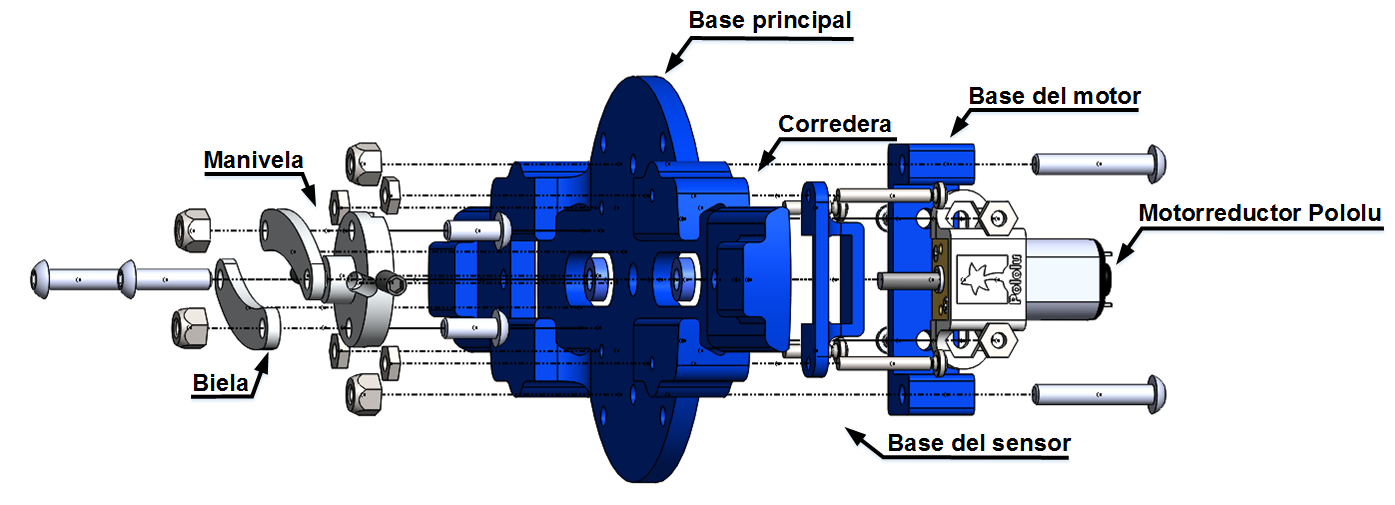
\includegraphics[scale=0.35]{imgmeca/Partesliberacion.png}  
		\caption{Elementos que conforman el SLVC.}
		\label{img:partesliberacion}
	\end{center}
\end{figure}


El SLVC es un mecanismo de biela-manivela-corredera doble. El motor de CD est� acoplado mec�nicamente a la biela: cuando el motor gira, la manivela mueve a la corredera. Las correderas est�n atoradas con la estructura del contenedor, por lo tanto, el veh�culo cient�fico se libera cuando las correderas se contraen. En la figura \ref{img:partesliberacion} se pueden ver los interruptores de extremos de carrera (puestos en las bases de sensor). El mecanismo tiene un interruptor de inicio de carrera en un lado y un interruptor de final de carrera en el otro. La figura \ref{img:slvcsecuencia} muestra la secuencia de activaci�n del mecanismo.

\begin{figure}[H]
	\begin{center}
		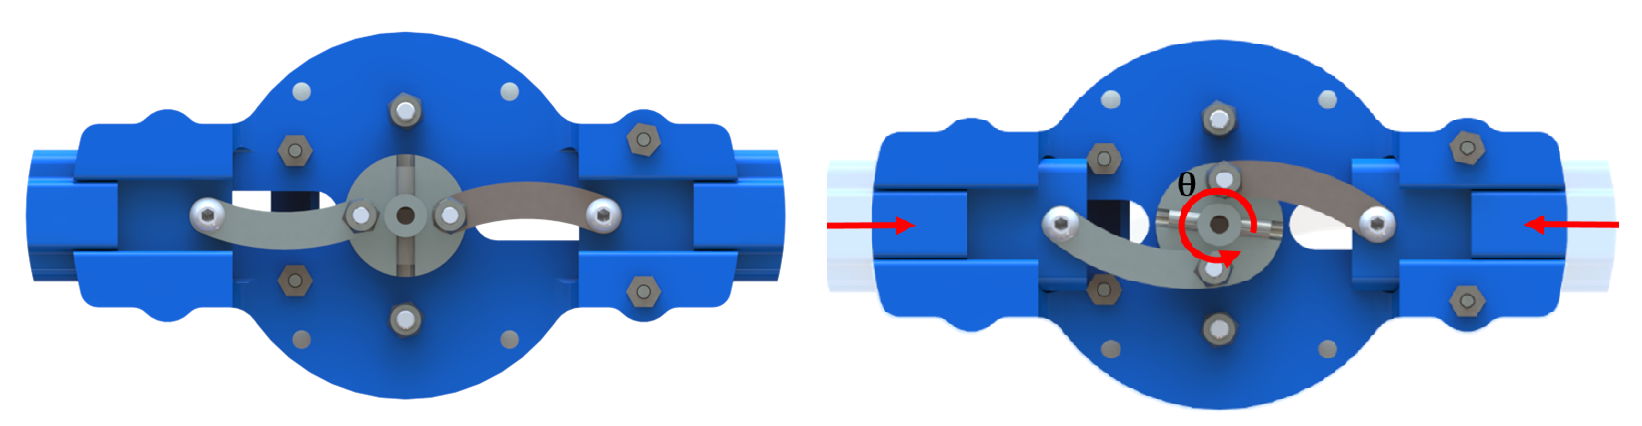
\includegraphics[scale=0.30]{imgmeca/SLVCsecuencia.png}  
		\caption{Secuencia de activaci�n del mecanismo del SLVC.}
		\label{img:slvcsecuencia}
	\end{center}
\end{figure}

Los interruptores de extremos de carrera son utilizados para obtener se�ales de retroalimentaci�n del movimiento del mecanismo. Dependiendo de qu� interruptor est� activado el microcontrolador puede determinar el estado del mecanismo: correderas extendidas (interruptor de final de carrera presionado) o correderas contra�das (interruptor de inicio de carrera presionado). Estas se�ales permiten activar el motor de CD por �nicamente el tiempo necesario, ahorrando energ�a de las bater�as.\\

\subsubsection*{Selecci�n de materiales}
Las manivelas y la biela son uno de los puntos m�s cr�ticos del mecanismo presentado en la figura \ref{img:partesliberacion} debido a que son los componentes que estar�n sometidos a flexi�n durante el despegue del CanSat. Por esta raz�n, la aleaci�n de aluminio AA 6061 fue seleccionada para su fabricaci�n, adem�s de ser una de las aleaciones m�s comunes. Las manivelas y la biela son piezas muy peque�as y, por lo tanto, no representan un valor de masa muy elevado.\\

Para el movimiento entre la base y las correderas se necesita poca fricci�n. Fabricar de aluminio estas piezas implicar�a mucha masa para el CanSat, por lo tanto, se utiliz� la impresi�n 3D con ABS. A las piezas impresas se les di� un tratamiento con vapor de acetona para eliminar la mayor cantidad de imperfecciones producidas por el proceso de deposici�n de material y as� reducir la fricci�n entre componentes.\\

}